\normaltrue \difficilefalse \tdifficilefalse
\correctiontrue
%\UPSTIidClasse{11} % 11 sup, 12 spé
%\newcommand{\UPSTIidClasse}{11}

\exer{Scooter Piaggio $\star\star$ \label{CHS:03:B2:16:81}}
%% 
\setcounter{question}{0}\marginnote{\xpComp{CHS}{03}}%\UPSTIcompetence[2]{B2-16}
\index{Compétence CHS-03}\index{Compétence B2-16}

\index{Scooter Piaggio}
\index{Hyperstatisme}

\ifcorrection
\else
\marginnote{\textbf{Pas de corrigé pour cet exercice.}}
\fi


\ifprof
\else
On s'intéresse au système direction du scooter Piaggio. 
La pièce 1 est composée des segments $G_1$ -- $O_1$ -- $D_1$.
La pièce 2 est composée des segments $G_2$ -- $O_2$ -- $D_2$.

\begin{figure*}[!h]
\centering
\begin{subfigure}[c]{.3\linewidth}
\centering
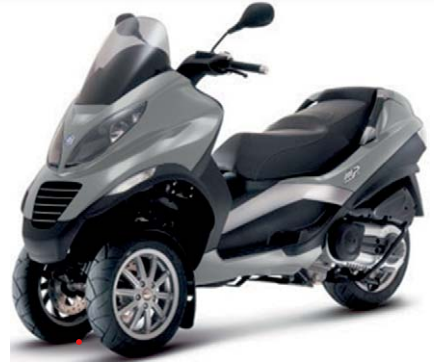
\includegraphics[height=4cm]{81_01.png}
\end{subfigure} \hfill
\begin{subfigure}[c]{.3\linewidth}
\centering
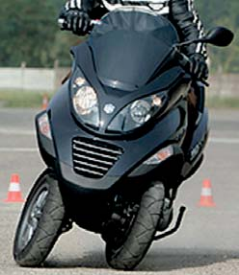
\includegraphics[height=4cm]{81_02.png}
\end{subfigure} \hfill
\begin{subfigure}[c]{.3\linewidth}
\centering
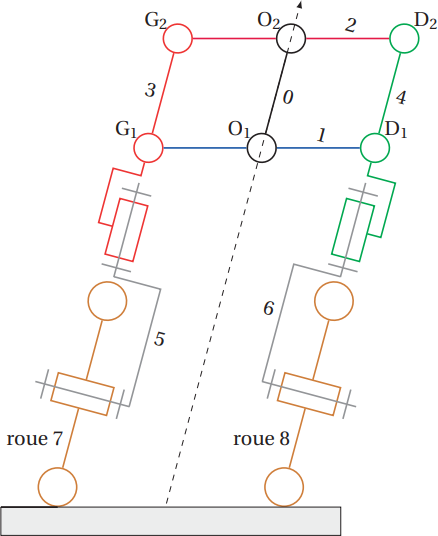
\includegraphics[height=5cm]{81_03.png}
\end{subfigure} 
\end{figure*}
\fi

\question{Réaliser le graphe de liaisons du système de direction. On considèrera le sol comme une classe d'équivalence.}
\ifprof
\begin{center}
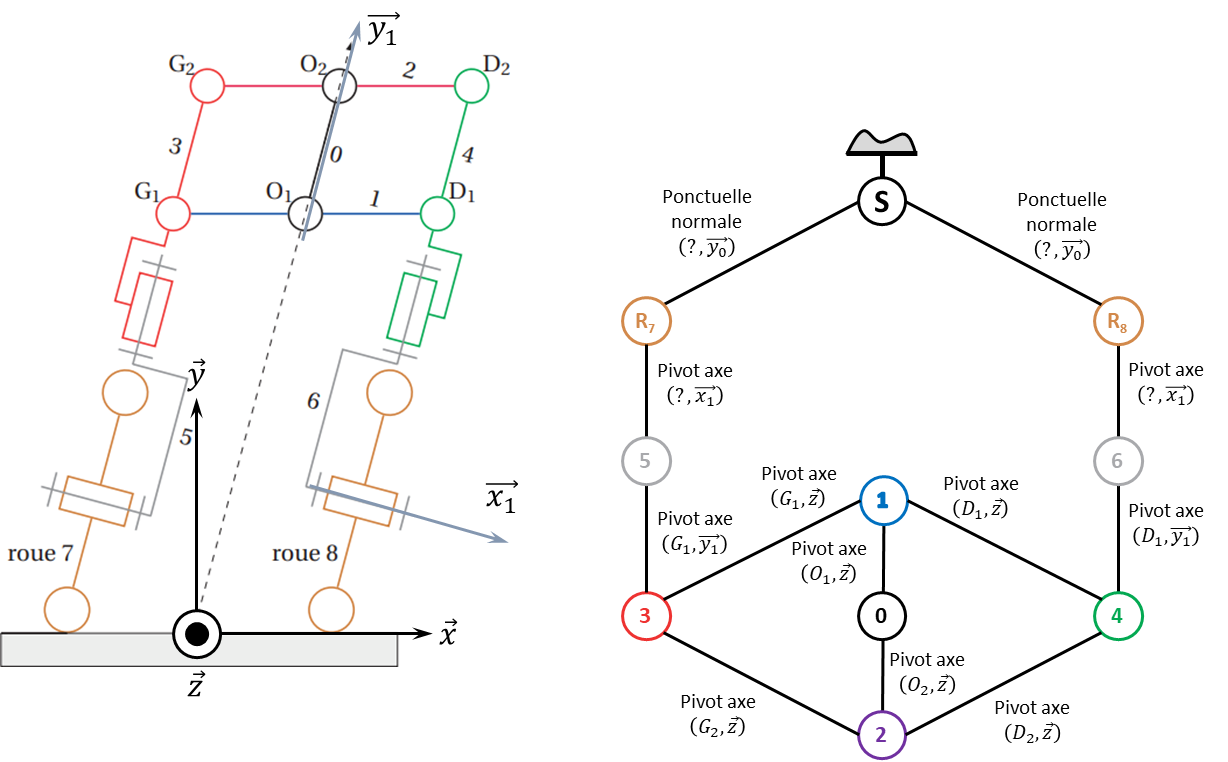
\includegraphics[width=.6\linewidth]{81_01_cor.png}
\end{center}
\else
\fi

\question{Calculer le degré d'hyperstatisme.}
\ifprof

\textbf{Méthode statique :}
\begin{itemize}
\item $h = m -E_s + I_s$ 
\item $m$ : rotation propre des roues 7 et 8 autour de $\vx{1}$, rotation des roues (7+5) et (6+8) autour de $\vy{1}$,  mouvement du parallèlogramme (1 rotatation), si toutes les liaisons pivots sont bloquées, il reste 2 ponctuelles en parallèle par rapport au sol, soit une liaison linéaire rectiligne (4 mobilités). Au final, $m=9$;
\item $E_S =9\times 6 = 54$;
\item $I_S = 10\times 5 + 2 \times 1 = 52$;
\item $h = 9 -54 + 52 = 7$.
\end{itemize}

\textbf{Méthode cinématique :}
\begin{itemize}
\item $h = m -I_c + E_c$ 
\item $m$ : cf ci-dessus. 
\item $E_c =3\times 6 = 18$;
\item $I_c = 10\times 1 + 2 \times 5 = 20$;
\item $h = 9 - 20 + 18 = 7$.
\end{itemize}


\else
\fi

\question{Si le modèle est hyperstatique, modifier le modèle pour le rendre isostatique.}
\ifprof
SI on considère l'ensemble 0,1,2,3,4 : 
\begin{itemize}
\item $h = m -E_s + I_s$ 
\item $m = 1$; 
\item $E_S =4\times 6 = 24$;
\item $I_S = 6\times 5  = 30$;
\item $h = 1 -24 + 30 = 7$. 
\end{itemize}
Tout l'hyperstatisme est donc concentré dans le double parallélogramme. 

On peut remplcer la pivot en $O_1$ par une linéaire annulaire, ce qui supprime 3 inconnues statiques. 
On peut aussi remplacer les pivots $G_2$ et $D_2$ par des rotules (supprimant ainsi 4 inconnues statiques).
\else
\fi
 

\ifprof
\else
\ifcolle\else
\marginnote{
\begin{solution}
\begin{enumerate}
\item .
\item $h=7$.
\item .
 \end{enumerate}
 \end{solution}
Corrigé  voir \ref{CHS:03:B2:16:81}.}

\fi
\fi